\documentclass[10.5pt]{config}
% 本实验报告采用 署名-相同方式共享 4.0 国际许可协议 (CC BY-SA 4.0)
\usepackage{multirow}
\usepackage{wrapfig}
\usepackage{setspace}
\usepackage{titlesec}
\usepackage{ctex}
\usepackage{graphicx} % 用于插入图片
\usepackage{float}    % 用于控制图片位置
\usepackage{makecell}
\usepackage{tikz}
\usetikzlibrary{arrows.meta}

\titleformat{\subsubsection}[block]  % 设置为块级标题（自动换行）
{\normalfont\bfseries}{\thesubsubsection}{1em}{} 
\titlespacing*{\subsubsection}{1.5em}{3.25ex}{1.5ex}  % 调整缩进：左缩进2em
\setstretch{1.5}

% --- 请在这里填写您的个人信息 ---
\major{机械工程} % 专业
\name{韩颂义}
\partner{} % 签名栏
\stuid{3240104198}
\date{2026.5.7} %
\lab{东3-308}
\grades{}
\course{电工电子学实验}
\instructor{季瑞松} % 指导老师
\exptype{基础实验} % 实验类型
\expname{集成运算放大器应用(一)} % 以PPT封面名称为准


\begin{document}

\makeheader % 首页头部

\section{实验目的}

\begin{enumerate}[label=\arabic*., leftmargin=2em]
    \item 了解集成运算放大器的基本使用方法和三种输入方式。
    \item 掌握集成运算放大器构成的比例、加法、减法、积分等运算电路的原理和功能。
\end{enumerate}

\section{实验设备}
\begin{enumerate}[label=\arabic*., leftmargin=2em]
    \item 模拟电子技术实验箱（带电源）
    \item 数字示波器
    \item 函数信号发生器
    \item 数字式万用表
\end{enumerate}

\section{实验原理}

集成运算放大器（简称集成运放）有同相输入、反相输入和差分输入三种信号输入方式。集成运放有线性放大和饱和（非线性）两种输出状态。为确保集成运放工作在线性放大区，电路必须引入负反馈。其实际引脚供电通常为 $\pm 12\mathrm{V}$ 双电源供电。

\subsection*{1. 同相输入比例运算电路}
当输入端加入信号 $u_i$ 时，在理想条件下，其输入输出的关系为：
\begin{equation*}
    u_o = \left( 1 + \frac{R_f}{R_1} \right) u_i
\end{equation*}

\begin{figure}[H] 
    \centering 
    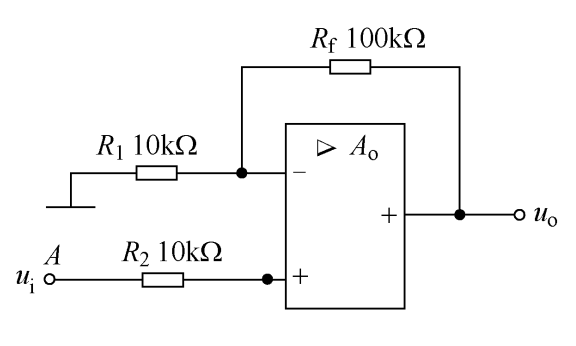
\includegraphics[width=0.45\textwidth]{figures/tongxiangdianlu.png} 
    \caption{同相输入比例运算电路}
    \label{fig:bili}
\end{figure}


\subsection*{2. 反相加法运算电路}
当输入端 A、B 加入 $u_{i1}$、$u_{i2}$ 信号时，其输出电压为：
\begin{equation*}
    u_o = -\left( \frac{R_f}{R_1} u_{i1} + \frac{R_f}{R_2} u_{i2} \right)
\end{equation*}

\begin{figure}[H] 
    \centering 
    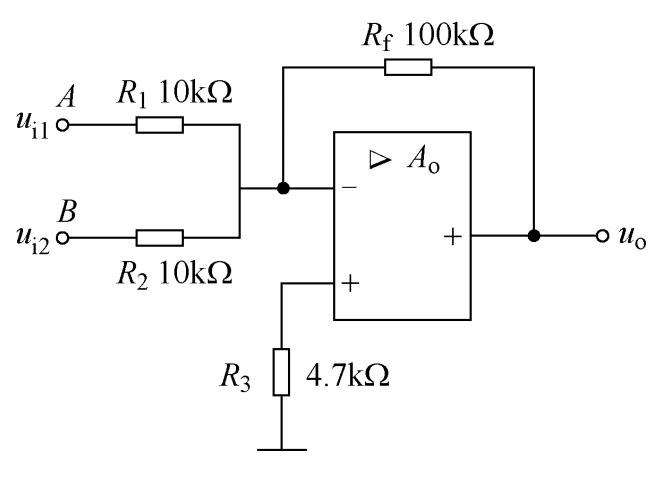
\includegraphics[width=0.45\textwidth]{figures/fanxiangdianlu.png} 
    \caption{反相输入比例运算电路}
    \label{fig:bili}
\end{figure}

\subsection*{3. 减法运算电路}
当输入端加入 $u_{i1}$、$u_{i2}$ 信号时，在理想条件下，且 $R_1 = R_2$、$R_f = R_3$ 时，其输出电压为：
\begin{equation*}
    u_o = \frac{R_f}{R_1} (u_{i2} - u_{i1})
\end{equation*}

\begin{figure}[H] 
    \centering 
    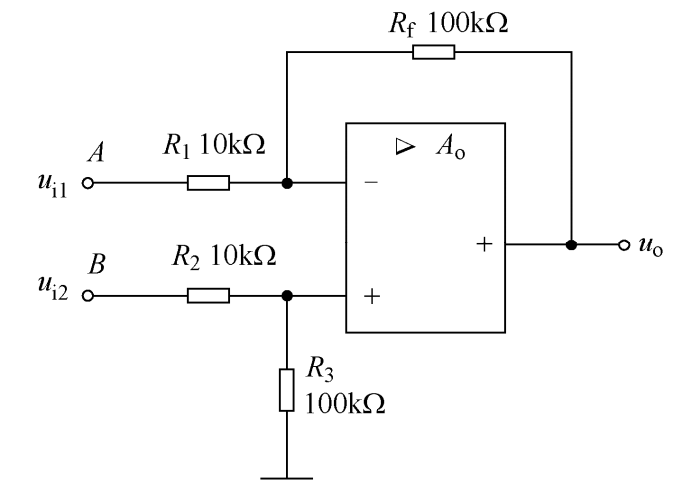
\includegraphics[width=0.45\textwidth]{figures/jianfadianlu.png} 
    \caption{减法运算电路}
    \label{fig:bili}
\end{figure}

\subsection*{4. 积分运算电路}
当开关 K 断开时，输入在 $t=0$ 时加入大小为 $U_i$ 的信号，若电容两端的初始电压为零，则输出为：
\begin{equation*}
    u_o = -\frac{1}{R_1 C} \int u_i \mathrm{d}t = -\frac{U_i}{R_1 C} t
\end{equation*}
当开关 K 闭合时，若输入信号 $u_i$ 的频率满足 $\omega \gg 1/R_2C$，则输出可近似为：
\begin{equation*}
    u_o \approx -\frac{1}{R_1 C} \int u_i \mathrm{d}t
\end{equation*}

\begin{figure}[H] 
    \centering 
    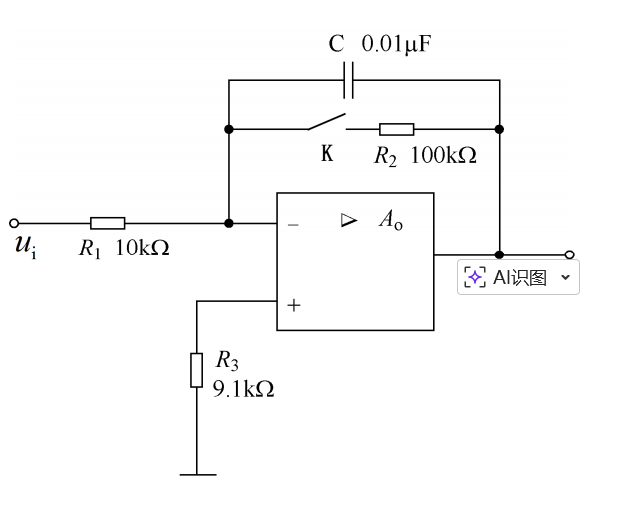
\includegraphics[width=0.45\textwidth]{figures/jifendianlu.png} 
    \caption{积分运算电路}
    \label{fig:bili}
\end{figure}

\section{实验内容}

\begin{enumerate}[label=\arabic*., leftmargin=2em]
    \item \textbf{同相输入比例运算电路：} 
    按图接线，输入峰值为 2V、频率为 100Hz 的正弦波。用示波器双踪观察输入和输出波形，记录示波器波形，根据波形计算比例系数。并用 x-y 模式记录传输特性曲线。（在 y-t 模式下，示波器双通道测量显示峰峰值和频率）
    
    \item \textbf{反相加法运算电路：} 
    按图接线，A 端输入峰值为 0.5V、频率为 1kHz 的方波，B 端输入峰值为 0.2V、频率为 1kHz 的三角波，要求方波超前三角波 $90^\circ$。用示波器的三个通道，同时观察 $u_{i1}$、$u_{i2}$ 和 $u_o$ 波形，确认电路功能正确并记录。
    
    \item \textbf{减法运算电路：}
    按图接线，A 端输入峰值为 3V、频率为 1kHz 的正弦波，B 端输入峰值为 2V、频率为 1kHz 的同相位正弦波。用示波器三通道同时观察 $u_{i1}$、$u_{i2}$ 和 $u_o$ 波形，确认电路功能正确并记录。

    \item \textbf{积分运算电路：}
    按图接线（K闭合），输入峰值为 2V，频率为 2kHz 的方波。用示波器双踪观察输入和输出波形，记录示波器波形。改变方波的频率为 200Hz 和 5kHz，分别观测输入和输出波形。
\end{enumerate}


\section{实验数据记录与波形}

% 请在此处替换为您实际在示波器上截图的波形图片
\begin{figure}[H] 
    \centering 
    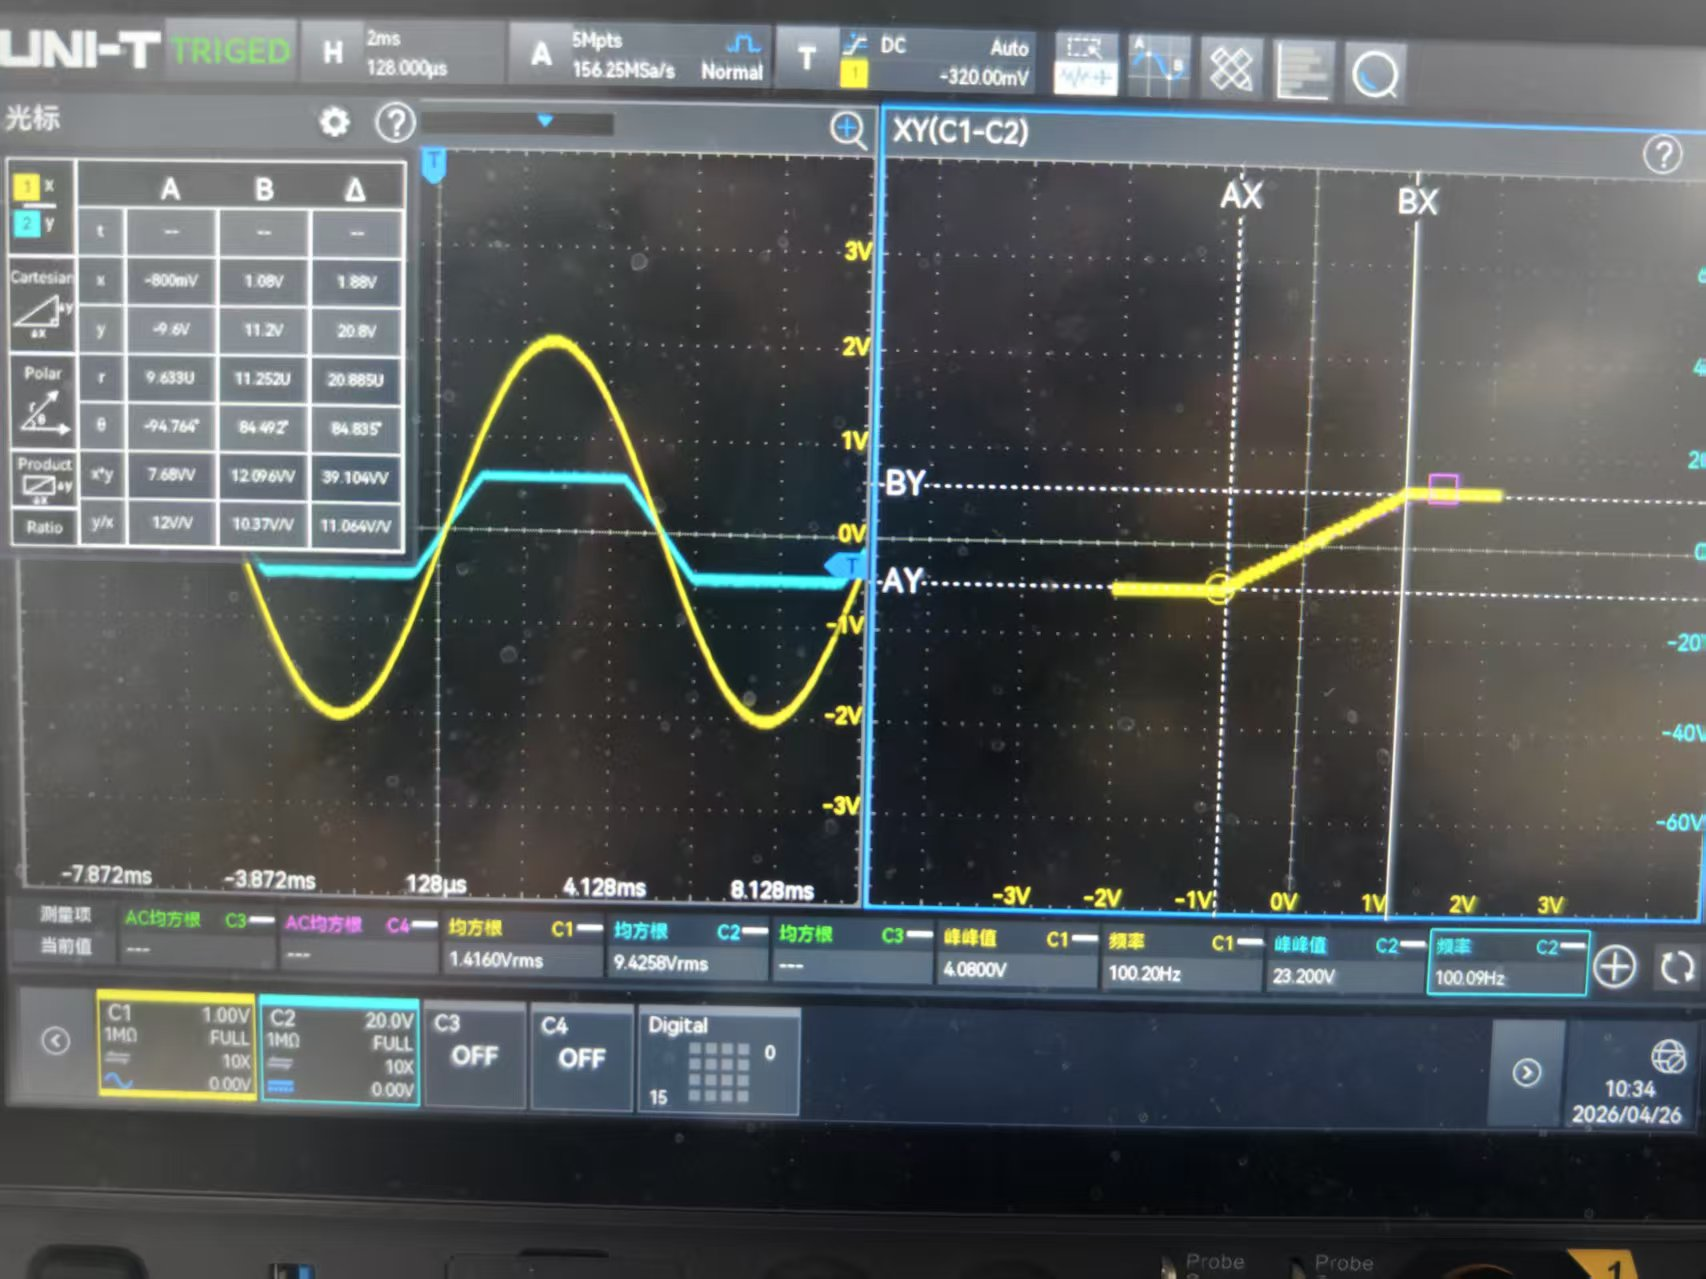
\includegraphics[width=0.45\textwidth]{figures/tongxiang.jpg} 
    \caption{同相输入比例运算波形 (y-t 模式与 x-y 模式)}
    \label{fig:bili}
\end{figure}

由图中读数读出，斜率约为11，即放大倍数约为11，这与理论计算结果$A_u = 1 + \frac{R_f}{R_1} = 1 + \frac{100\text{k}\Omega}{10\text{k}\Omega} = 11$相同




\begin{figure}[H] 
    \centering 
    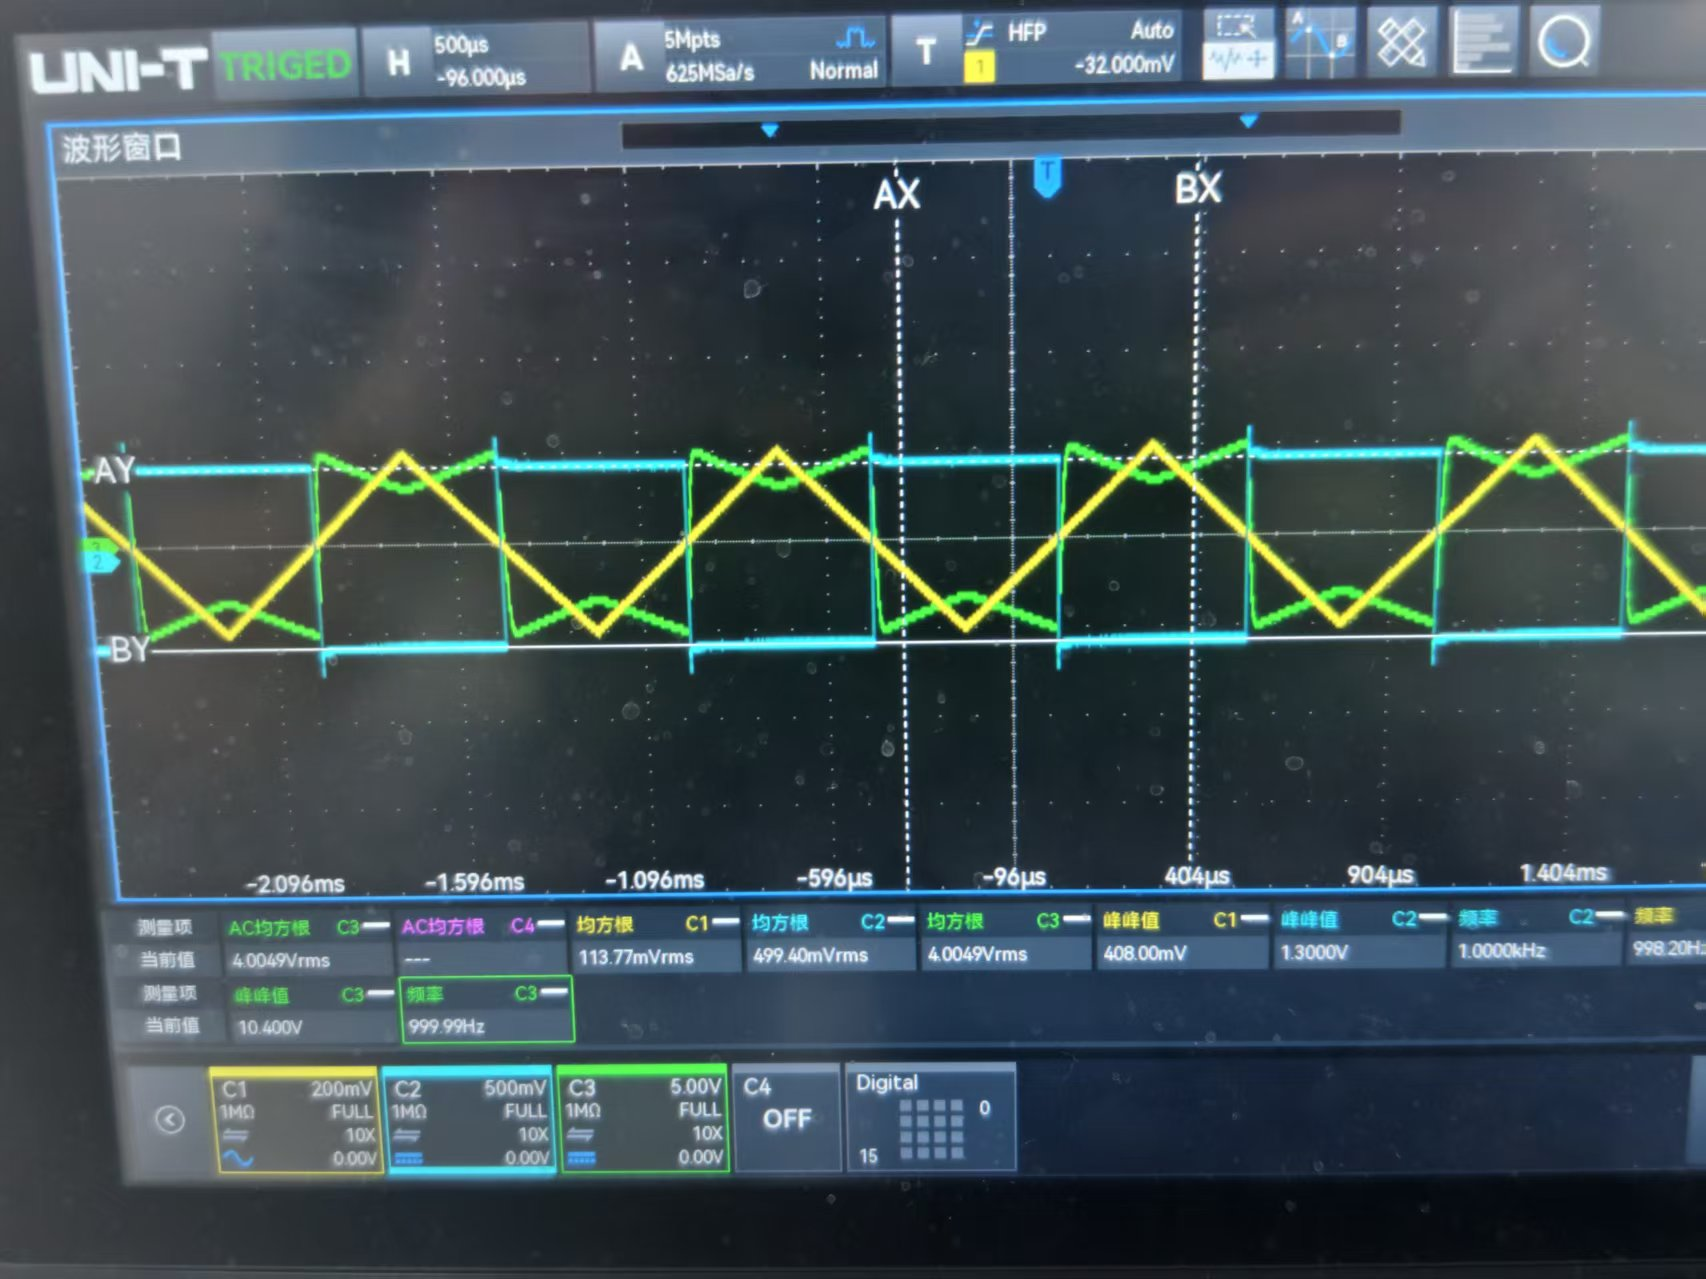
\includegraphics[width=0.45\textwidth]{figures/lan.jpg} 
    \caption{加法运算波形-输入信号1}
    \label{fig:jianfa}
\end{figure}


\begin{figure}[H] 
    \centering 
    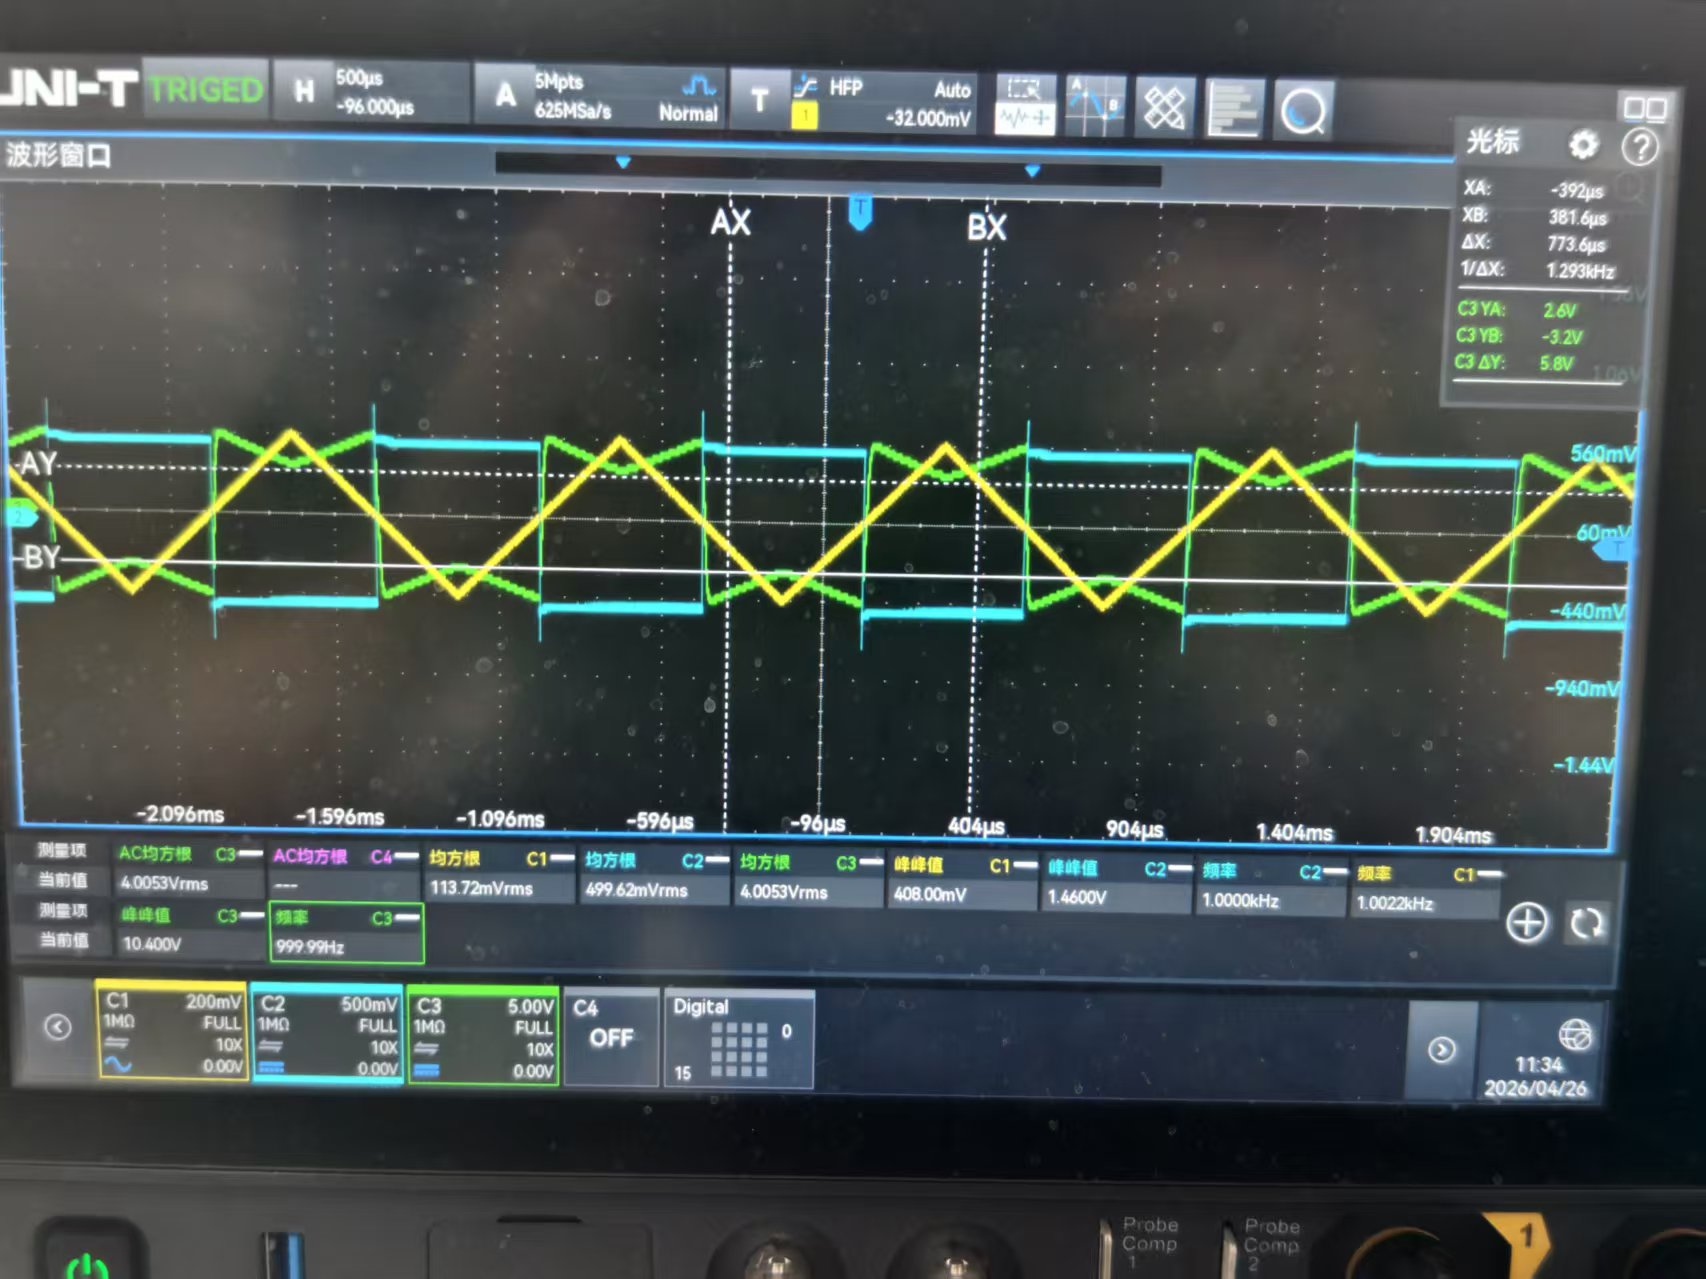
\includegraphics[width=0.45\textwidth]{figures/huang.jpg} 
    \caption{加法运算波形-输入信号2}
    \label{fig:jianfa}
\end{figure}

\begin{figure}[H] 
    \centering 
    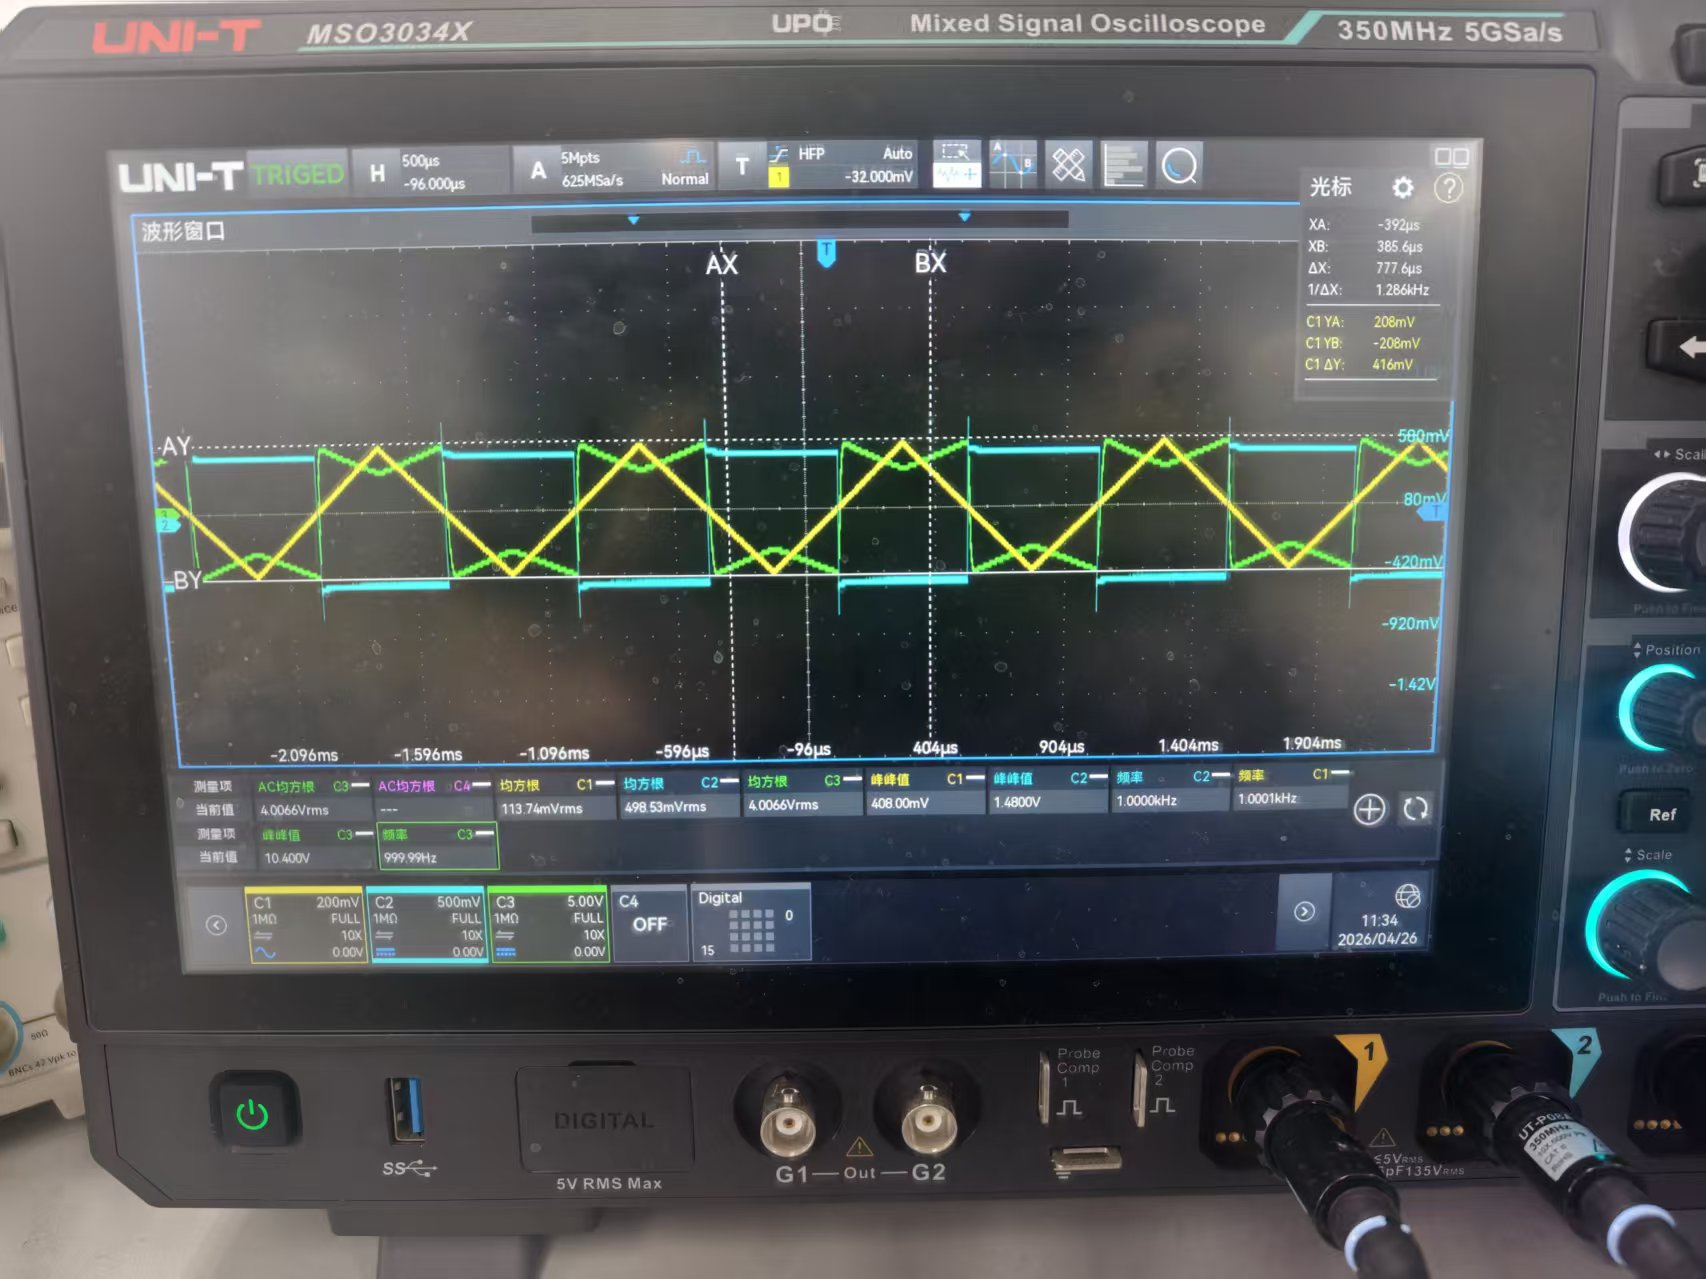
\includegraphics[width=0.45\textwidth]{figures/lv.jpg} 
    \caption{加法运算波形-输出信号}
    \label{fig:jianfa}
\end{figure}


由图中读数可见，当输入信号 $u_{i1} = 0.5\text{V}$（方波）、$u_{i2} = -0.2\text{V}$（三角波负尖峰）时，输出信号极小值约为 $2.9\text{V}$。这与理论计算结果吻合，推导公式如下：
\begin{equation*}
    u_o = -\left( \frac{R_f}{R_1}u_{i1} + \frac{R_f}{R_2}u_{i2} \right) = -\left[ \frac{100}{10} \times 0.5 + \frac{100}{10} \times (-0.2) \right] = -3\text{V}
\end{equation*}



\begin{figure}[H] 
    \centering 
    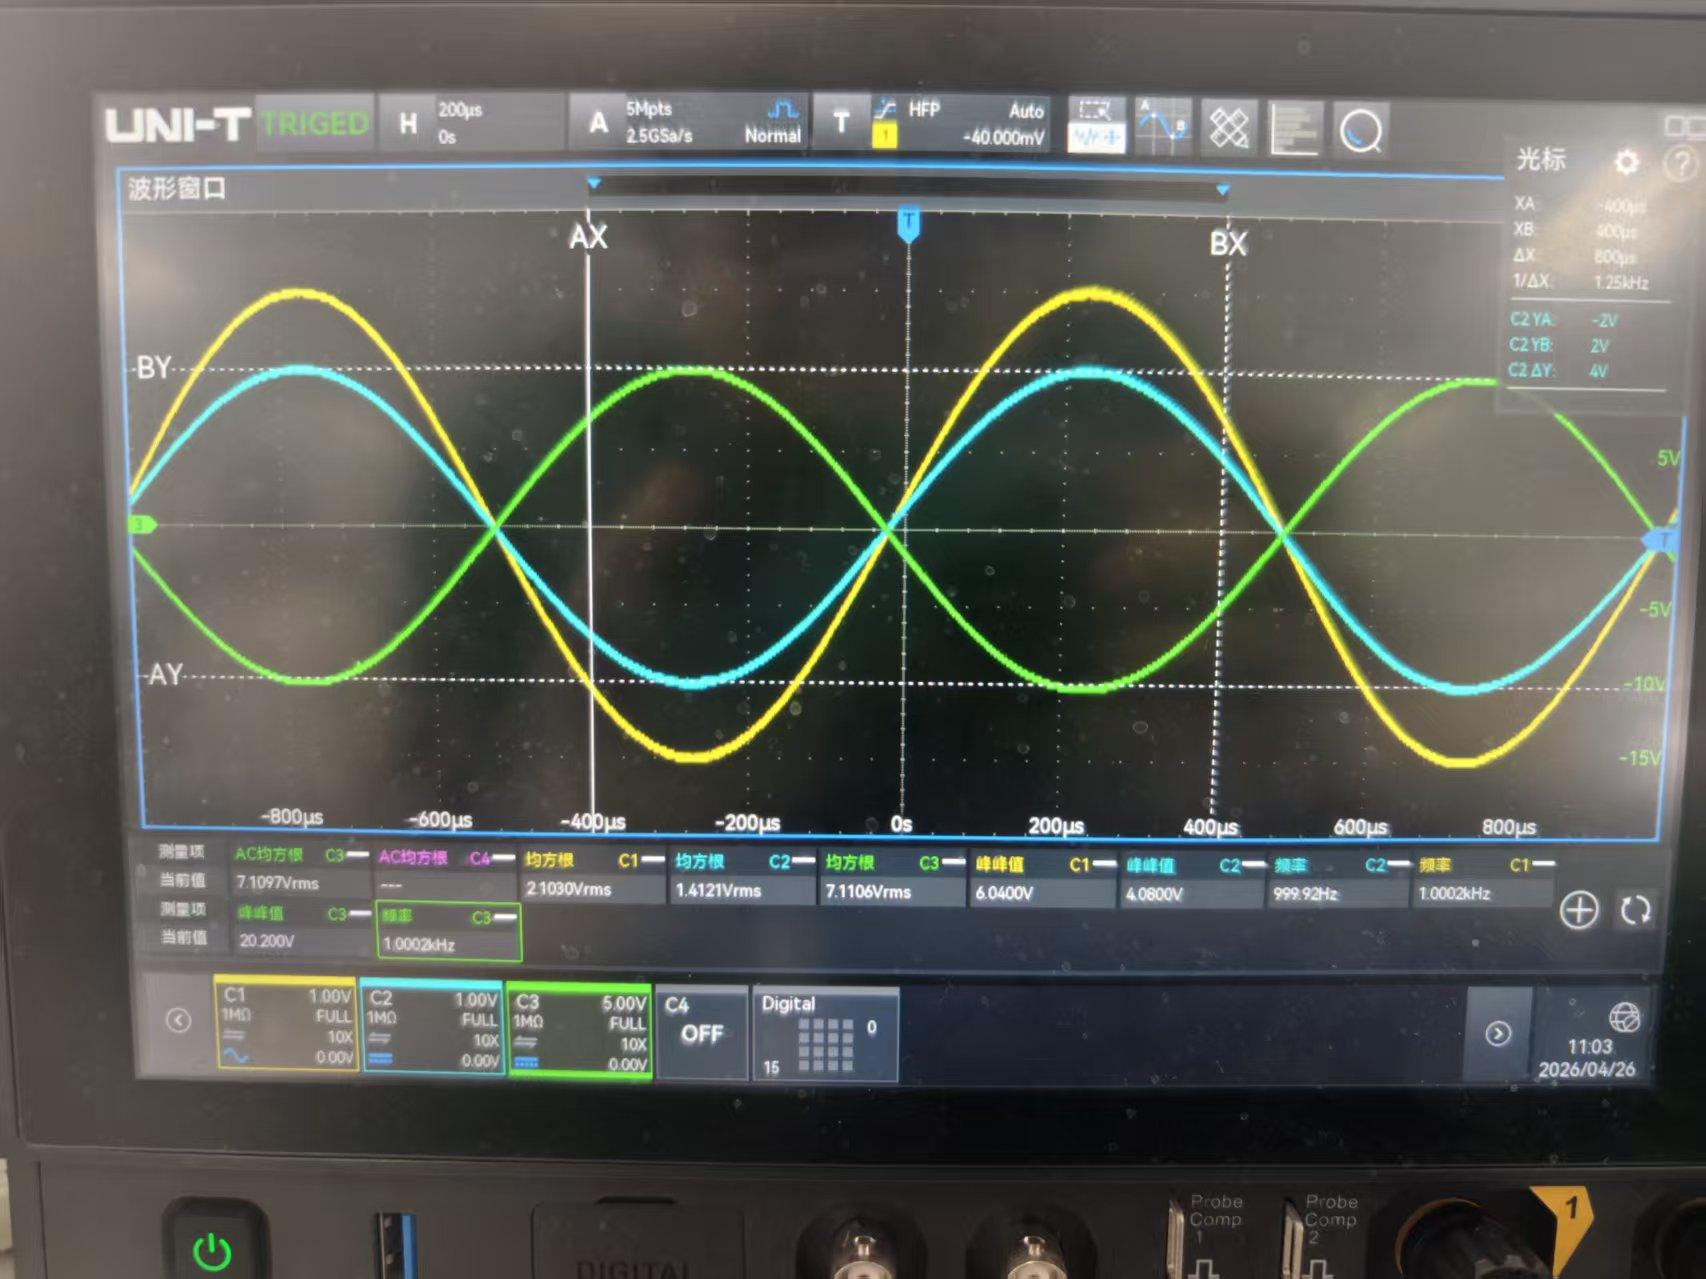
\includegraphics[width=0.45\textwidth]{figures/jianfa.jpg} 
    \caption{减法运算波形 (三通道)}
    \label{fig:jiafa}
\end{figure}
由图中读数得出，$u_{i1} = 3.02\text{V}$，$u_{i2} = 2.04\text{V}$，实测输出电压幅度 $|u_o| = 10.1\text{V}$。这与理论计算结果基本吻合。
在反相加法电路中，理论计算公式如下：
\begin{equation*}
    u_o = -\left( \frac{R_f}{R_1}u_{i1} + \frac{R_f}{R_2}u_{i2} \right) = -(10 \times 3.02 - 10 \times 2.04) = -9.8\text{V}
\end{equation*}


\begin{figure}[H] 
    \centering 
    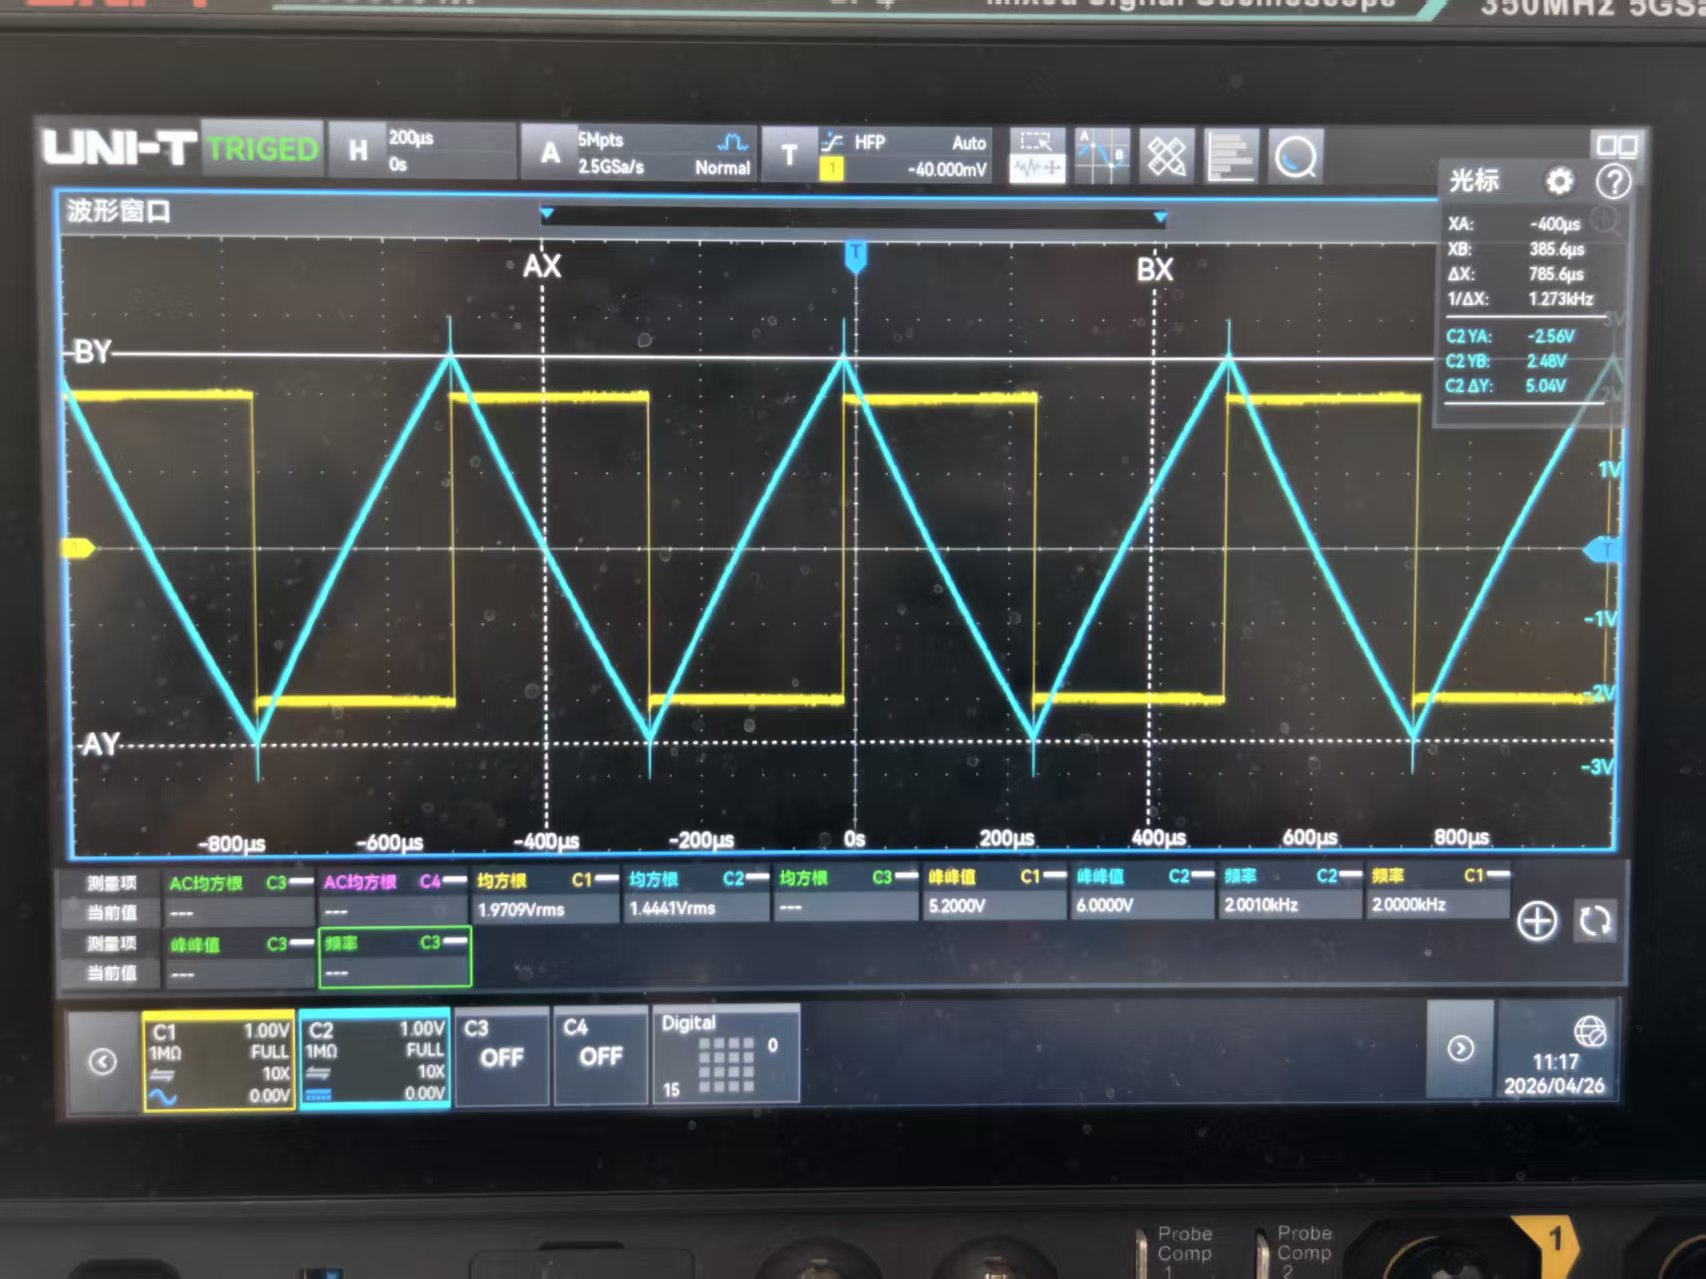
\includegraphics[width=0.45\textwidth]{figures/jifen2k.jpg} 
    \caption{积分运算波形 (2kHz 方波输入)}
    \label{fig:jifen}
\end{figure}

\begin{figure}[H] 
    \centering 
    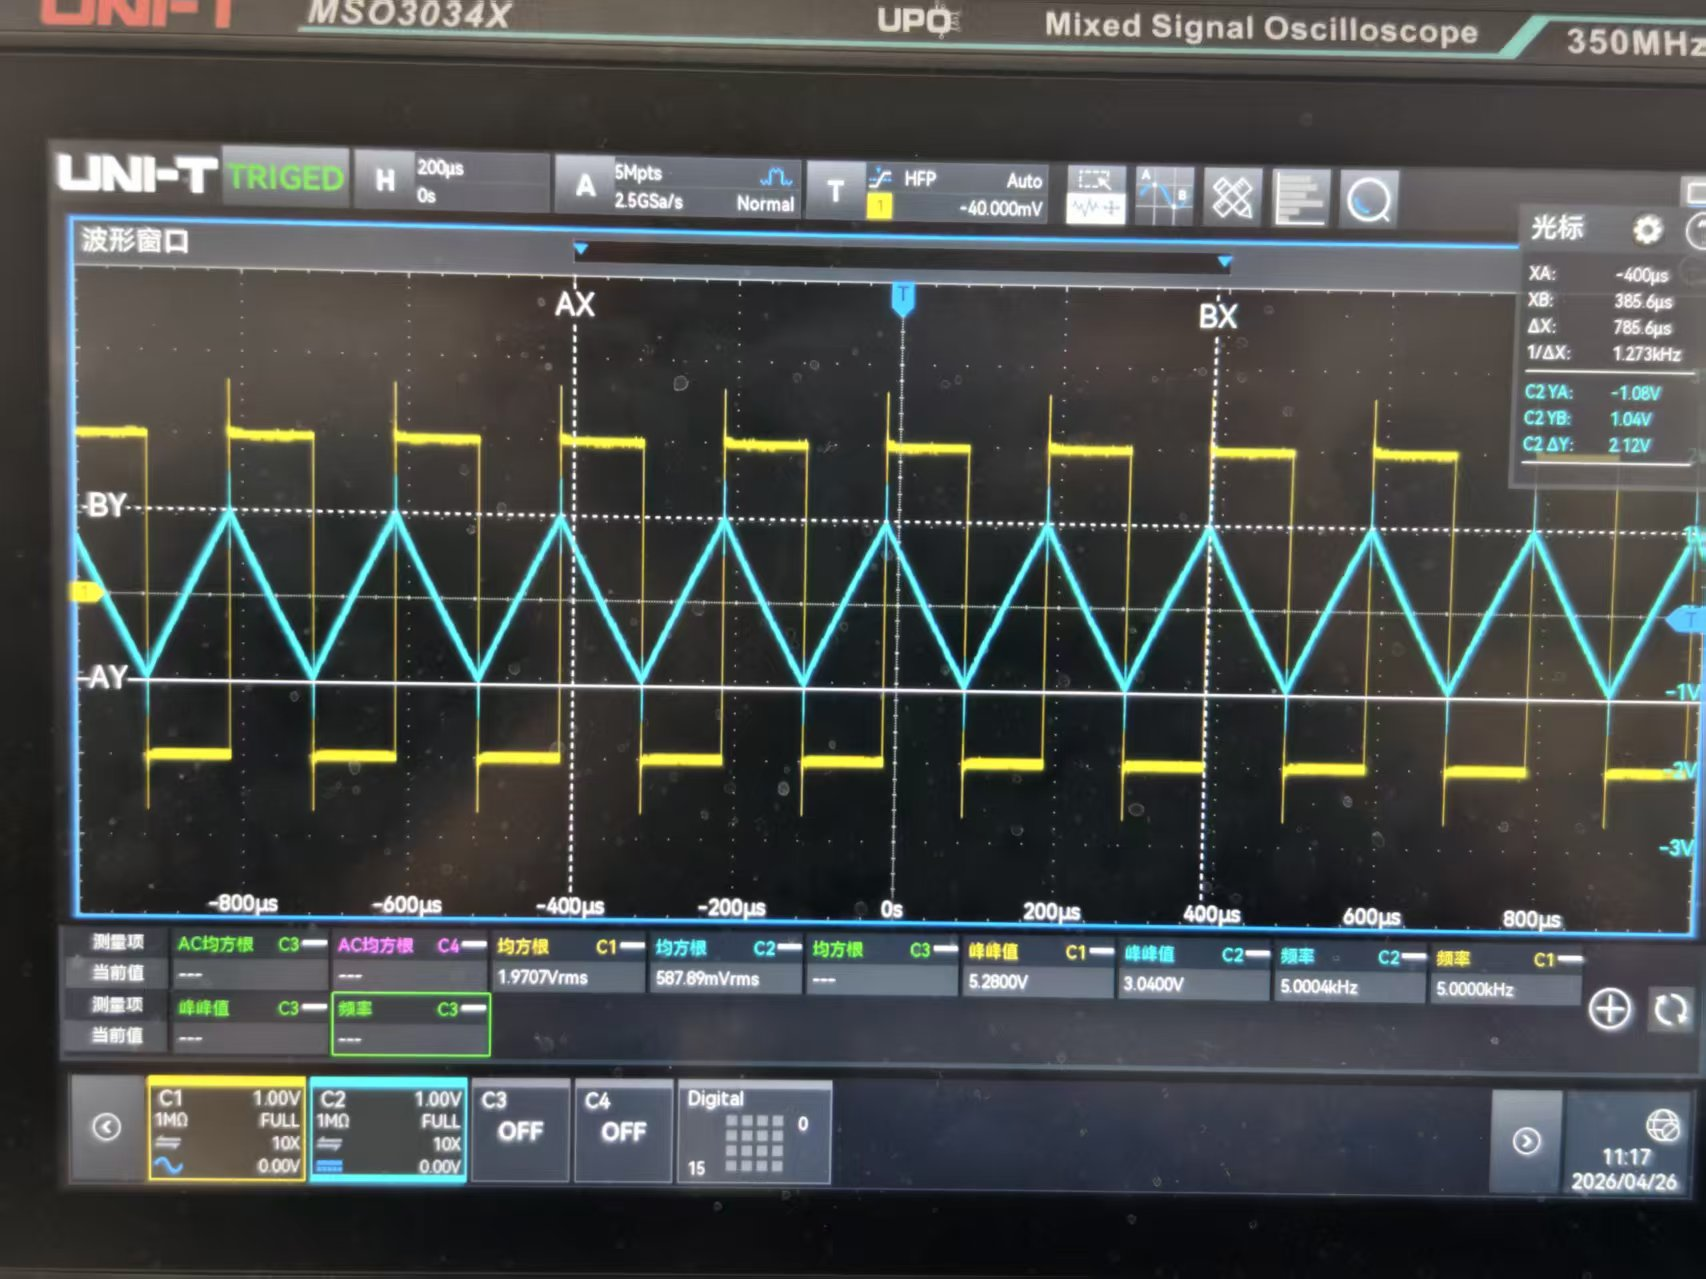
\includegraphics[width=0.45\textwidth]{figures/jifen5k.jpg} 
    \caption{积分运算波形 (5kHz 方波输入)}
    \label{fig:jifen}
\end{figure}

\begin{figure}[H] 
    \centering 
    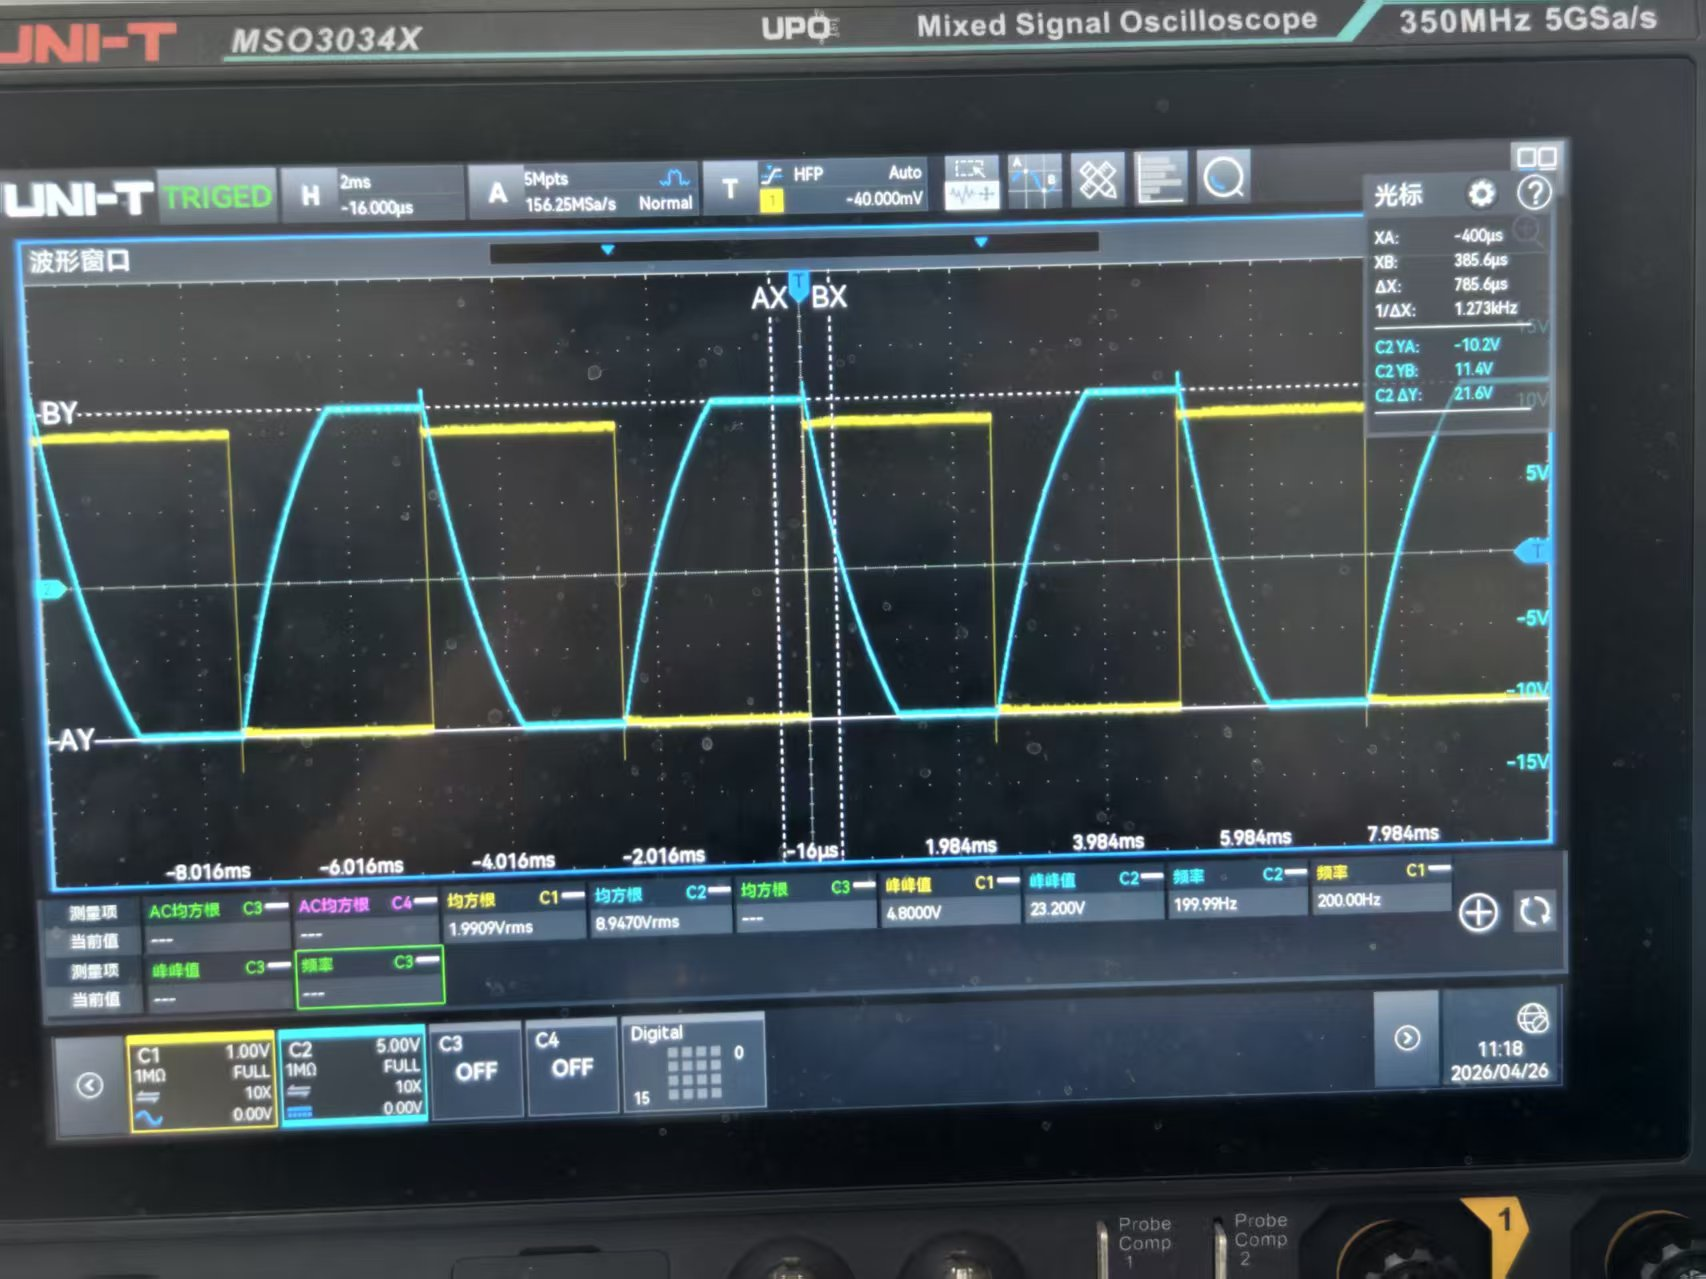
\includegraphics[width=0.45\textwidth]{figures/jifen100.jpg} 
    \caption{积分运算波形 (100Hz 方波输入)}
    \label{fig:jifen}
\end{figure}


\section{实验总结}

\subsection*{第一部分：思考题解析 (P168 四、1. 2. 3.)}
\begin{enumerate}[label=\arabic*., leftmargin=2em]
    \item \textbf{推导各电路表达式：}
    在深度负反馈且理想运放条件下，满足“虚短”($u_+ = u_-$)和“虚断”($i_+ = i_- = 0$)。
    \begin{itemize}
        \item 同相比例：$u_+ = u_i$，由于虚短 $u_- = u_i$。流过 $R_1$ 的电流为 $u_- / R_1$，流过 $R_f$ 的电流为 $(u_o - u_-) / R_f$。由虚断知两电流相等，得 $u_o = (1 + R_f/R_1)u_i$。
        \item 反相加法：$u_+ = 0$ (接地)，$u_- = 0$ (虚地)。节点电流方程：$u_{i1}/R_1 + u_{i2}/R_2 + u_o/R_f = 0$，解得 $u_o = -(R_f/R_1 \cdot u_{i1} + R_f/R_2 \cdot u_{i2})$。
        \item 减法：利用叠加定理，当 $u_{i1}$ 作用时为反相比例，当 $u_{i2}$ 作用时为同相比例，两者相加且在 $R_1=R_2, R_f=R_3$ 条件下可得 $u_o = (R_f/R_1)(u_{i2}-u_{i1})$。
        \item 积分：反相端虚地，$u_-=0$。输入电流 $i = u_i / R_1$。电容电流 $i_C = - C (\mathrm{d}u_o/\mathrm{d}t)$。两者相等积分得 $u_o = -\frac{1}{R_1 C} \int u_i \mathrm{d}t$。
    \end{itemize}
    \item \textbf{输出电压会无限增大吗？为什么？}
    不会。集成运放的输出电压受限于其直流供电电源电压（本实验中为 $\pm 12\mathrm{V}$）。随着输入电压或积分时间的增大，一旦计算出的理论输出超过电源电压范围，运放内部的三极管将进入饱和区，输出电压会被钳位在接近电源电压的最大输出幅度（如 $\pm 10\mathrm{V} \sim \pm 11\mathrm{V}$ 左右），此时电路处于非线性工作状态，波形出现平顶失真。

\item \textbf{根据指导书要求及图 5.16-3 所示加法定标电路参数：}



\begin{itemize}[leftmargin=2em]
    \item 输入电压变化范围：下限 $U_{il} = -1\mathrm{V}$，上限 $U_{ih} = -5\mathrm{V}$
    \item 输出电压变化范围：下限 $U_{ol} = 0\mathrm{V}$，上限 $U_{oh} = 10\mathrm{V}$
    \item 电路固定参数：直流基准电源 $U_{CC} = 15\mathrm{V}$，输入端电阻 $R = 10\mathrm{k}\Omega$
\end{itemize}


根据加法定标电路的原理，要求当输入达到下限 $u_i = U_{il}$ 时，输出 $u_o = 0\mathrm{V}$。由公式可得：
\begin{equation*}
    R_1 + R_{p1} = -\frac{U_{CC}}{U_{il}} R
\end{equation*}
代入已知数据进行计算：
\begin{equation*}
    R_1 + R_{p1} = -\frac{15\mathrm{V}}{-1\mathrm{V}} \times 10\mathrm{k}\Omega = 150\mathrm{k}\Omega
\end{equation*}

同理，要求当输入达到上限 $u_i = U_{ih}$ 时，输出 $u_o = U_{oh}$。由公式可得：
\begin{equation*}
    R_2 + R_{p2} = \frac{U_{oh}}{U_{il} - U_{ih}} R
\end{equation*}
代入已知数据进行计算：
\begin{equation*}
    R_2 + R_{p2} = \frac{10\mathrm{V}}{-1\mathrm{V} - (-5\mathrm{V})} \times 10\mathrm{k}\Omega = \frac{10\mathrm{V}}{4\mathrm{V}} \times 10\mathrm{k}\Omega = 25\mathrm{k}\Omega
\end{equation*}



\end{enumerate}

\subsection*{第二部分：实验结果分析与体会}
\begin{itemize}[leftmargin=2em]

        \item \textbf{运算电路定量分析与误差评价：}
        通过对各项实验数据的对比，可以发现实测值与理论推导值高度吻合。
        \begin{itemize}
            \item \textbf{同相比例电路：} 实测斜率约为 11，与由 $1+R_f/R_1$ 计算出的理论倍数完全一致，验证了同相放大器的高输入阻抗与相位一致性。
            \item \textbf{反相加法电路：} 当方波与三角波叠加时，实测极小值为 $2.9\text{V}$，与理论值 $3\text{V}$ 的误差仅为 3.3\%。
            \item \textbf{减法电路：} 实测输出 $10.1\text{V}$，理论计算为 $9.8\text{V}$，误差在合理范围内。
        \end{itemize}
    
        \item \textbf{积分电路的时域特性探究：}
        积分实验生动地展示了 $RC$ 时间常数与输入信号频率对输出波形的影响：
        \begin{itemize}
            \item 在低频（$100\mathrm{Hz}$）时，由于积分时间过长，输出电压极易达到饱和值，波形呈现明显的截幅现象；
            \item 在中频（$2\mathrm{kHz}$）时，输出为线性度较好的三角波；
            \item 在高频（$5\mathrm{kHz}$）时，积分时间变短，根据 $u_o = -\frac{1}{RC}\int u_i dt$，输出三角波的幅值明显减小，但线性度（斜率稳定性）得到进一步提升。这证明了积分电路在信号变换与波形整形中的关键作用。
        \end{itemize}


    \item \textbf{运算电路功能特点总结：}
    通过实验观测，\textbf{同相比例电路}实现了信号的同相放大，输入阻抗高；\textbf{反相加法电路}能够将多路信号（方波与三角波）线性反相叠加，互不干扰；\textbf{减法电路}有效提取了两路同频正弦波信号的差值；\textbf{积分电路}则成功地将输入的方波信号转换为了三角波信号。积分电路的波形受频率影响显著：频率越高，积分条件满足得越好，三角波线性度越高但幅度越小。
    
    \item \textbf{输入电压对工作状态的影响：}
    在 x-y 模式下观察同相比例电路的电压传输特性曲线时可以直观看到，当输入电压幅值较小（居中区域）时，特性曲线为一条斜率恒定的直线，运放处于\textbf{线性工作状态}，实现正常的数学运算；而当输入信号幅值过大时，曲线两端变为水平线，运放进入\textbf{饱和状态（非线性工作状态）}，失去线性运算功能。
    
    \item \textbf{实验体会与问题解决：}
    实验中遇到了一些问题，首先是芯片坏掉了，好在一开始就有排查的习惯及时更换；第二个是 示波器对峰峰值的读数不准，这个主要是波形会有一些毛刺，比如一些过冲，导致示波器将其当做最高点。本次实验还是收获满满的，让我直观地体会到运放是如何工作的。

\end{itemize}



\end{document}